\chapter{Formalism}\label{chap:Formalism}

I will use this chapter to cover several important mathematical concepts which are required for the reader to understand the advantages and disadvantages of computational sensing. I will first discuss the advantages that Hadamard and S-Matrix multiplexing provide compared to the isomorphic sensor to create a context for the discussion of the Fellgett advantage. Then I will discuss \acrfull{pca}, a technique for finding useful discriminating features from seemingly complicated data. I will also cover the fundamentals of Bayesian statistics and how is can be used to update one's belief in a hypothesis given new data. Then will I cover important topics in compressive sensing: sparsity, incoherence, and the \acrfull{rip} and discuss an optimization problem that allows one to reconstruct sparse signals from compressively sampled data. 

To simplify the math and notation, I shall try to work with discrete representations of signals when possible. Any discrete linear process can be written as a matrix multiplication
%
\begin{equation}
	\mb{g} = \mb{H}\mb{f} + \mb{e}	
\label{eq:gHf}
\end{equation}
%
where \gls{measvec} is a vector of measurement data and \gls{objvec} is a discrete representation of the object signal-of-interest and $\mb{H}$ is the matrix which describes the measurement process and \gls{noisevec} is additive noise. For brevity I will refer to \gls{objvec} as the object and $\mb{H}$ as either the sensing matrix or the measurement matrix. \Cref{eq:gHf} represents the forward model in a wide variety of computational sensors. The object \gls{objvec} is a vector in $N$ dimensional vector space and the measurement \gls{measvec} is a vector in $N_m$ dimensional vector space. In general $N_m \neq N$. 

\Cref{eq:gHf} is an extremely useful way to represent optical phenomena, since it allows one to take advantage of many attractive numerical techniques which are dedicated to linear systems. For the most part, classical optics---the ray and wave nature of light---can be approximated a linear. 
The solutions to the paraxial wave equation are linear in free space and in most glasses. Similarly, paraxial optics can be model using a sequence of matrix multiplications. While just an approximation, tracing the paraxial Chief and Marginal ray is enough to calculate the third-order Seidel aberrations. 



\section{Isomorphic Sensing}

In an isomorphic measurement, where the goal is a one-to-one mapping of object points to measurement points, the measurement matrix is represented with the identity matrix
\begin{equation}
	\mb{H}=\mb{I}	
\end{equation}

One can get an idea of how much error exists in an isomorphic measurement by invoking the weighing example \cite{harwit2012hadamard}. Say there are $4$ objects with true unknown weights $f_{1}, f_{2}, f_{3}, f_{4}$. The measured weights are $g_{1}, g_{2}, g_{3}, g_{4}$ with additive noise  $ e_1, e_2, e_3, e_4 $. 
\begin{equation}
	\left[ \begin{matrix} g_1\\ g_2\\ g_3\\ g_4\end{matrix} \right] = \left[ \begin{matrix} 1& 0& 0& 0\\ 0& 1& 0& 0\\ 0& 0& 1& 0\\ 0& 0& 0& 1\end{matrix} \right] \left[ \begin{matrix} f_1\\ f_2\\ f_3\\ f_4\end{matrix} \right] + \left[ \begin{matrix} e_1\\ e_2\\ e_3\\ e_4\end{matrix} \right] 
	\label{eq:gHfpluse}
\end{equation}
Since this is \gls{isomorphic sensing}, the estimated weights \gls{estobjvec} are the measurements  $ \mathbf{g} $
\begin{equation}
	\mathbf{ \hat{ f }} = \mathbf{g}. 
\end{equation}
Where the error between the estimated weights and the actual weights is $ \mb{\epsilon} = \mbh{f} - \mb{f} $. For simplicity, I assume a zero mean distribution for the noise. Therefore, the isomorphic measurements are unbiased.\footnote{Unbiased means that on average the estimator will produce the ground truth} For an unbiased estimator, the \gls{mse} of the estimated weights is the variance
\begin{equation}
	E [  \mb{\epsilon} ^2 ] = E [ ( \mbh{f} - \mb{f} )^2 ] = \sigma^2.
\end{equation}
This puts a lower bound on the \gls{mse} for an isomorphic measurement. 

\section{Multiplexing}

As I discussed in \Cref{chap:Introduction}, \gls{multiplexing} is a technique for overcoming \gls{snr} related trade-offs in \gls{isomorphic} sensing. In a multiplexed measurement, each element in the measurement vector \gls{measvec} is a weighted linear combination of the elements in the object vector. Therefore the measurement matrix $\mb{H}$ is no longer an identity matrix. 

\subsection{Coding Schemes}\label{subsec:codingschemes}

A Hadamard matrix of order $N$ is defined as a matrix \gls{hadamardn} as the $N \times N$ matrix whose elements consist of $+1$'s and $-1$'s and satisfies the following property:
\begin{equation}
	\mb{H}_{N}^T \mb{H}_{N} = \mb{H}_{N} \mb{H}_{N}^T = N \mb{I}_{N}
\end{equation}
where $\mb{I}_N$ is an $N \times N$ identity matrix. 

In computational spectroscopy and imaging, Hadamard codes are extremely popular. Hadamard codes are provably optimal in the case where one is allowed to take a full set of measurements, meaning that \gls{objvec} and \gls{measvec} from \Cref{eq:gHf} are both vectors in $N$ dimensional space \cite{harwit2012hadamard}. 

A Hadamard multiplexed measurement is written as
%
\begin{equation}
\left[ \begin{matrix} g_{1}\\ g_{2}\\ g_{3}\\ g_{4}\end{matrix} \right] =\left[ \begin{matrix} +1 +1 +1 +1 \\ +1 -1 +1 +1 \\ +1 -1 -1 +1 \\ +1 -1 -1 +1 \end{matrix} \right] \left[ \begin{matrix} f_{1}\\ f_{2}\\ f_{3}\\ f_{4}\end{matrix} \right]
\end{equation}
%
In the weighing example, negative measurements are realized by using a balancing scale instead of a spring scale. This means that in the first measurement all 4 items are placed in the same pan. In the second measurement items 1 and 3 are in the same pan while items 2 and 4 are in the opposite pan, and so on \cite{harwit2012hadamard}. With four equations and four unknowns, one can solve for the estimates using basic algebra.

The \gls{mse} of the $m^{th}$ measurement  
\begin{equation}
	E [ ( \hat{f}_{m} - {f}_{m} )^2 ] = \frac{1}{4} \sigma^2.
\end{equation}
which is $4$ times lower than using an isomorphic measurement scheme. In general, the \gls{mse} of a Hadamard measurement is 
\begin{equation}
	\text{MSE} = \frac{\sigma^2}{N}
	\label{eq:hadamardmse}
\end{equation}
where $N$ is the dimension of the object vector $\mb{f}$, which is equal to the number of measurements \gls{nummeas}. Hotelling proved in 1944 that for a measurement matrix with elements $h_{mn} \in \{-1, +1\}$, the lowest possible MSE for the case of a full set of measurements with a linear unbiased estimator is $\text{MSE} = \frac{\sigma^2}{N}$ \cite{brady2009optical}. Therefore, one cannot possibly do better than Hadamard coding in this case. 

In many practical cases in computational sensing, making a code with simultaneous positive and negative modulation of the signal is not possible. While this may be possible using incoherent light where a phase delay maybe used to produce a negative electric field. For incoherent light, the system response is linear in intensity \cite{goodman2005introduction}. 

In the case where one has the ability to make a full set of measurements but is limited to elements of $+1$'s and $0$'s, an S-Matrix code minimizes the \gls{mse} \cite{harwit2012hadamard}. In the weighing example, a spring balance rather than a two pan scale analogous to this situation. 
\begin{equation}
\left[ \begin{matrix} g_{1}\\ g_{2}\\ g_{3}\\ g_{4}\end{matrix} \right] = 
\left[ \begin{matrix} 0 & +1 & +1 & +1 \\ +1 & +1 & 0 & 0 \\ +1 & 0 & +1 & 0 \\ +1 & 0 & 0 & +1 \end{matrix} \right]
\left[ \begin{matrix} f_{1}\\ f_{2}\\ f_{3}\\ f_{4}\end{matrix} \right]
\end{equation}
So items 2, 3, and 4 are weighed together, then 1 and 2, and so on. Solving the system of equations in a silimar fashion as before in the Hadamard weighing example we find that the mean square error for the $m^{th}$ measurement when weighing 4 items is 
\begin{equation}
\text{MSE} = E [ ( \hat{f}_{m} - {f}_{m} )^2 ] = \frac{7}{9} \sigma^2.
\end{equation}
Which reduced the \gls{mse} compared to the \gls{isomorphic} measurement scheme but has higher \gls{mse} compared to the Hadamard measurement scheme. The \gls{mse} of the S-Matrix is approximately a factor of 4 increase compared to the Hadamard matrix coding scheme. 

In the case when the full set of measurements are available $\ap{N_m = N}$, I have just shown that Hadamard codes are optimal. It would seem as if random coding would have no use if one is able to utilize Hadamard codes. However, they should not be ignored because in compressive sensing, certain theoretical guarantees exist for random coding that do not exist for Hadamard and S-Matrix codes. Sometimes, the physics of the situation forces a random coding scheme. 

\subsection{The Fellgett Advantage}

The \gls{Fellgett advantage} is the improvement in \gls{snr} that occurs when an instrument takes multiplexed measurements compared to isomorphic measurements \cite{fellgett1958principes, davis2001fourier}. Physically the \gls{Fellgett advantage}  occurs because a single detector element produces a noise contribution whether it is sampling a single part of the signal or multiple parts of the signal. Maximizing the \acrfull{snr} of the estimated object signal-of-interest for a given system throughput and detector noise is major design consideration in computational optical sensing particularly in the area of spectroscopy. There are two notable ways to accomplish multiplexing in spectroscopy: Hadamard multiplexing in dispersive spectrometers and interferometric based multiplexing such as the \gls{fts}. 

The \gls{fts} architecture is a similar to the Michelson interferometer, see Figure \ref{fig:fourierTransformSpec}. The \gls{fts} operates by taking the autocorrelation of the complex electric field as a function of time delay by moving one of the mirrors in the interferometer \cite{davis2001fourier}. The Wiener-Khinchin theorem says that for a wide-sense stationary random process, the Fourier transform of the autocorrelation is the power spectral density \cite{goodman2015statistical}. Thus a computational post-processing step is required to reconstruct the spectrum from the measured autocorrelation data. Since the \gls{fts} measures combinations of multiple wavelengths at each detector readout, it also exhibits the \gls{Fellgett advantage}. It turns out that in a \gls{fts} the \gls{mse} obtained is a factor of two greater than the Hadamard multiplexing spectrometer \cite{tai1976fourier}. 

\begin{equation}
	\text{MSE} = 2 \frac{\sigma^2}{N_{\lambda}} 
\end{equation}
%
where $N_{\lambda}$ is the number of spectral channels. 
%
\begin{figure}
	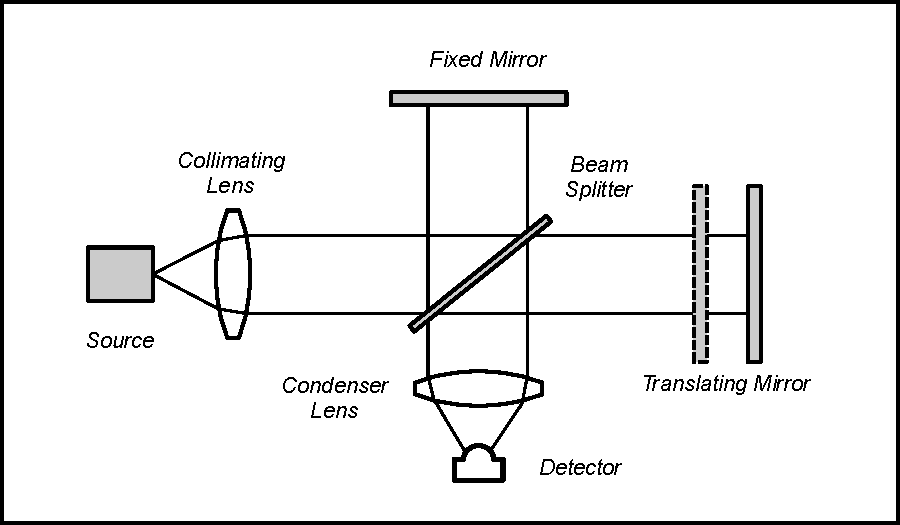
\includegraphics[scale=1]{fourierTransformSpec}
	\captionof{figure}[The architecture of the Fourier Transform Spectrometer.]{The architecture of the Fourier Transform Spectrometer resembles the Michelson interferometer. One of the mirrors is translated back and forth. The interferogram is the detected intensity versus mirror delay which is related to the autocorrelation of signal. The Fourier transform of the autocorrelation provides the spectrum.}
	\label{fig:fourierTransformSpec}
\end{figure}

\section{Principal Component Analysis}

Principal component analysis (PCA) is a technique that attempts to recast a dataset in manner that finds correlations in data that may not be evident in their native basis and creates a set of basis vectors in which the data has a low dimensionalpoints al representation. \Gls{pca} works by producing a set of vectors that point along the direction of maximum variance while being simultaneously orthogonal to each other. These are called the \emph{principal components}. The first principal component vector is parallel to the direction of maximum variance. The second principal component points in the direction that also maximizes variance but is orthogonal to the first principal component. The third principal component is orthogonal to the first and second principal components and points in the direction that maximizes the variance given those constraints. And so on. 

Imagine one has a dataset $\mb{S}$ which consists of $N$ spectra with \gls{numspecchan} spectral channels. Instead of looking at the data as just intensity versus spectral channel, \gls{pca} attempts to construct a set of new vectors (also called features) that show as much variation in the spectra as possible. In other words, first direction (principal component) is used to recast the data to look as different (uncorrelated) as possible. This allows us to discriminate the data, as best we can with just one direction. The second principal component is the direction that provides the second most ability to discriminate the data, and so on. 

Now I will discuss some of the math behind \gls{pca}. The covariance matrix is defined as
\begin{equation}
\mb{C_{\mb{S}}} = \frac{1}{N} \mb{S} \mb{S}^{T}.
\end{equation}
%
Each element in the covariance matrix $C_{\mb{s}mn}$ is the covariance of the $m^{th}$ spectrum $\mb{s}_m$ and the $n^{th}$ spectrum $\mb{s}_n$. 
%
\begin{equation}
C_{\mb{s}mn} = \frac{1}{N} \mb{s}_m \mb{s}_n^{T}.
\end{equation}
%
A large covariance means they look alike and therefore are difficult to disambiguate. Geometrically, it means that $\mb{s}_m$ and $\mb{s}_n$ tend to point in the same direction (assuming their length is approximately the same). If the entire collection of spectra $\mb{S}$ were mutually orthogonal, being able to tell one spectrum apart from another would be easy. You would just have a collection of spikes at different spectral channels. The covariance matrix in this case would be a diagonal matrix. Therefore, it is desirable to have covariance matrices that are diagonal matrices since they indicate low correlation between the datasets and improves one's ability to distinguish between the data.

Since there is typically some redundancy between spectra, the off-diagonal elements of the covariance matrix will be non-zero. \Gls{pca} allows one to recast the data to make it as uncorrelated as possible in a new basis. 
\begin{equation}
	\mb{Y} = \mb{PS}
\end{equation}
where $\mb{Y}$ is the data projected onto the principal component basis $\mb{P}$. The \emph{rows} of matrix $\mb{P}$ are the principal components.  The covariance of the projected data
\begin{equation}
	\mb{C_{Y}} = \frac{1}{N} \mb{Y} \mb{Y}^{T} 
\end{equation}
is a now diagonal matrix. Indeed, the principal components are the optimal way to discriminate the spectra in the dataset \cite{jolliffe2002principal}. It turns out the principal components are the \emph{eigenvectors of the covariance matrix $\mb{C}_{\mb{S}}$ are the principal components} \cite{shlens2014tutorial}. 

Since the full set of principal components forms a basis, each spectra $\mb{s}$ in $\mb{S}$ can be written as a superposition of principal components without any error
\begin{equation}
\mb{s} = \sum_{n = 1}^{N_{\lambda}} \gamma_{n} \mb{p}_{\lambda}
\end{equation}
Where $\gamma_{n}$ is the $n^{th}$ eigenvalue associated with eigenvector $\mb{p}_{n}$. In many cases, only a few of the first principal components are needed in the summation to approximate the original data well, $M \ll N_{\lambda} $. Note that each eigenvector has an associated eigenvalue. The eigenvalues are also informative because the relative magnitude of the eigenvalue can tell us how many principal components are really needed to discriminate all of the spectra \cite{poon2009image}. The magnitude of the eigenvalue $\gamma_{n}$ tells us how well useful the associated eigenvector is at discriminating the data.


This is another reason why \gls{pca} is so useful. It can be used as a way to perform dimensionality reduction. In other words, seemingly complicated data can be summarized by only for few principal components by exploiting the correlations between the data. This concept is analogous to lossy compression in signal processing. Simply project the data onto the first several principal components associated with the largest $M$ eigenvalues. The data now has an approximately sparse representation. 

In will show in \Cref{chap:Afssic}, that the \gls{afssi-c} relies on a variation of Principal Component Analysis (PCA) for discriminating between spectra. In addition to \gls{pca}, the AFSSI-C uses a Bayesian technique to create adaptive codes. I will now discuss some of fundamentals of Bayesian statistics. 

\section{Bayesian Statistics}

A hypothesis is nothing more than a claim or premise that one is interested in verifying. In imaging and spectroscopy, one example is that at a certain location in the field of view, the hypothesis is that a spectrum is present. Another hypothesis is that the mean value of the signal is some value. Often times one is interested in estimating parameters of stochastic processes, which we denote $\theta$. 

Bayesian statistics allows one to treat the hypothesis or parameters as random variables rather than deterministic constants. At the heart of Bayesian approaches is Bayes' theorem, which is a way of computing probabilities of a hypothesis given some evidence which are related to the hypothesis. For example, Bayes' theorem can be used to decide which of two bags of candy has been opened or if a spectrum is present. The idea is that one  can make a more informed calculation of probability if one is able to update the probability given some new piece of evidence that one may have not had at the beginning.

The derivation of Bayes' theorem follows from the definition of conditional probability. The conditional probability of event $A$ occurring given that $B$ occurred is:

\begin{figure}
	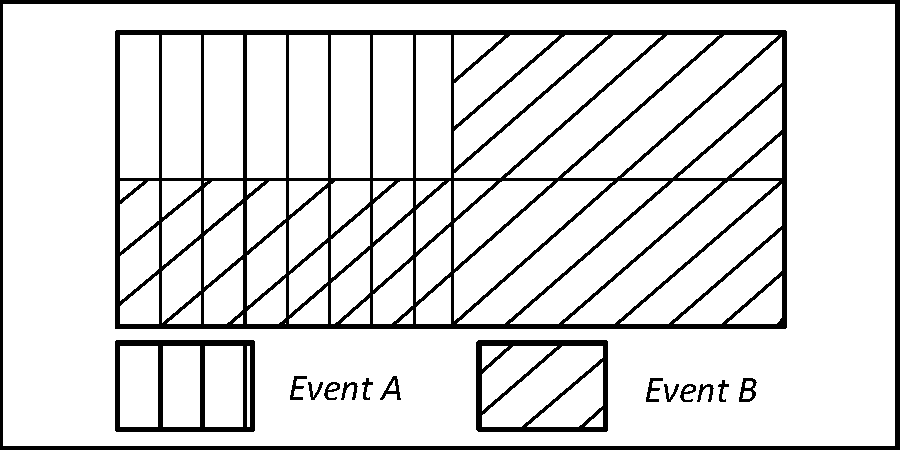
\includegraphics[scale=1]{definitionOfConditionalProbability}
	\captionof{figure}[Graphical demonstration of joint probability.]{Graphical demonstration of joint probability. The probability of event $A$ is $P(A)=3/4$. The probability of event $B$ is $P(B)=3/4$. The joint probability of events $A$ and $B$ is $P(A \cap B) = 1/4$. The probability of event $A$ occuring given that event $B$ has occured is $P( A \given B) = 1/3$. This is consistent with the equation $ P(A \cap B) = P(A \given B) P(B) $}
	\label{fig:definitionOfConditionalProbability}
\end{figure}

\begin{equation}
	P \left( A \given[\big] B \right) = \frac{ P \left( A \cap B \right) }{ P \left( B \right)}
\end{equation} 
%
this can be seen graphically in \Cref{fig:definitionOfConditionalProbability}. Solving for the joint probability $ P \left( A \cap B \right) $ gives
%
\begin{equation}
 P \left( A \cap B \right) =	P \left( A \given[\big] B \right)  P \left( B \right)
\label{eq:bayeStep2}
\end{equation} 
%
since the joint probability commutes $ P \left( A \cap B \right) = P \left( B \cap A \right) $, we can also write
%
\begin{equation}
 P \left( A \cap B \right) =	P \left( B \given[\big] A \right)  P \left( A \right)
\label{eq:bayeStep3}
\end{equation} 
%
equating the right hand sides of Equation \ref{eq:bayeStep2} and Equation \ref{eq:bayeStep3} gives use Bayes' theorem (also called Bayes' rule)
%
\begin{equation}
	P \left( A \given[\big] B \right) = \frac{ P \left( A \right) P \left( B \given[\big] A \right) }{ P \left( B \right) } 
	\label{eq:BayesTheoremBoxed}
\end{equation}
%
One interpretation of Bayes' theorem is called the Diachronic interpretation, which says that conditional probability of the hypothesis or parameter given knowledge of some evidence or measurement data is given by 

\begin{equation}
	P \left( \theta \given[\big] g \right) = \frac{ P \left( \theta \right) P \left( g \given[\big] \theta \right) }{ P \left( g \right) }
	\label{eq:diachronic}
\end{equation}

The term $ P \left( \theta \given[\big] g \right) $ is called the \gls{posterior}. It represents the belief in the hypothesis given the data. The term $ P \left( \theta \right) $ is called the \gls{prior}. $P \left( g \given[\big] \theta \right)$ is called the \gls{likelihood}. $P \left( \theta \right)$ is called the normalizing constant, which computed to ensure that the posterior probabilities sum to $1$.  The normalizing constant can be written as 
\begin{equation}
P \left( \theta \right) = \sum_{i} P \left( \theta_i \right) P \left( g_i \given[\big] \theta_i \right)
\label{eq:normalizingConstant}
\end{equation}
One can repeatedly apply Bayes' theorem given new measurement data. 

\subsection{Example: Updating Probabilities with Bayes' Theorem}

\begin{figure}
	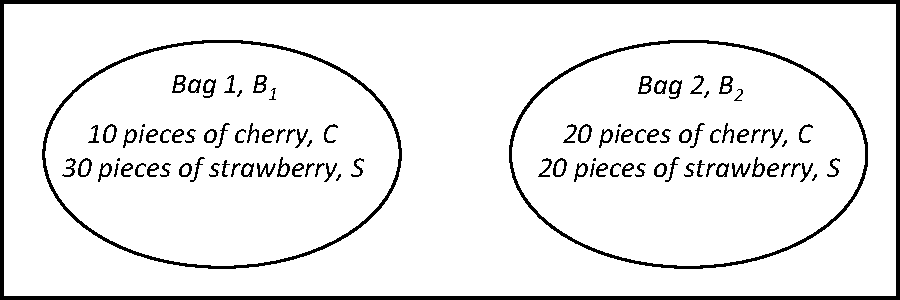
\includegraphics[scale=1]{candyExample}
	\captionof{figure}[Candy example for updating probabilities with Bayes' theorem]{Two bags are present: $B_1$ and $B_2$. The probability of choosing either bag is $P(B_1) = P(B_2) = 1/2$. Bag 1 has 40 pieces of candy: 10 pieces of cherry candy so $P(C|B_1) = 1/4$ and 30 pieces of strawberry so $P(S|B_1) = 3/4$. Bag 2 has 40 pieces of candy: 20 pieces of cherry candy so $P(C|B_2) = 2/4$ and 20 pieces of strawberry so $P(S|B_2) = 2/4$. If someone selects one of the bags at random then selects a piece of candy from that bag. If the candy is identified but the bag is not, then one can use Bayes' theorem to update the probability of either bag being selected. }
	\label{fig:candyExample}
\end{figure}

I will use a simple example to illustrate how to update probabilities using Bayes' theorem, see \Cref{fig:candyExample}. Imagine I have two bags of candy, Bag 1, which I denote $B_1$, and Bag 2, which I denote $B_2$. Bag 1 has 10 pieces of cherry flavored candy, denoted as $C$, and has 30 pieces of strawberry flavored candy, denoted as $S$. Bag 2, $B_2$, has 20 pieces of cherry candy and 20 pieces of strawberry candy. At the beginning, the prior probability of selecting bag 1 or bag 2 is both equal
%
\begin{equation}
	P \left( B_1 \right) = P \left( B_2 \right) = \frac{1}{2}
\end{equation}
%
Someone then picks a bag at random and takes out a piece of candy that turns out to be strawberry flavor. They do not state which bag was selected, only that the candy they randomly selected from the bag was strawberry. What is the probability that bag 1 was the one selected given that I know the candy is strawberry? I can use Bayes' theorem to compute this
%
\begin{equation}
	P \left( B_1 \given[\big] S \right) = \frac{ P \left( B_1 \right) P \left( S \given[\big] B_1 \right) }{ P \left( S \right) }
\end{equation}
%
$ P \left( S \given[\big] B_1 \right) $ is the probability of selecting strawberry given that they pick bag 1, which is $3/4$. $ P \left( S \right) $ is the probability of selecting a strawberry candy from either bag 1 or bag 2, which $5/8$. Thus
%
\begin{equation}
	P \left( B_1 \given[\big] S \right) = \dfrac {\left( \dfrac {1} {2}\right) \left( \dfrac {3} {4}\right) } {\left( \dfrac {5} {8}\right) } = \frac{3}{5}
\end{equation}
%
Similarly, the probability that the person chose bag 2 is $P \left( B_2 \given[\big] S \right) = 2/5$. Qualitatively, this makes sense, since bag 1 contained more strawberry flavored candy, the probability that bag 1 was chosen should increase since it has more strawberry candy and the probability that bag 2 was chosen should decrease.

Now to continue the example. Imagine the first piece of candy is put back into the bag from where it came from. Then another piece of candy is drawn from the same bag, which turns out to be cherry flavor. Now one must update the probabilities with this new piece of information. One can keep using Bayes' theorem. The posteriors from the last draw $m-1$ are now used as the priors for the current update.

\begin{equation}
	P \left( B_1 \given[\big] C \right)_{ m } = \frac{ P \left( C \given[\big] B_1 \right) P \left( B_1 \given[\big] S \right)_{m-1} }{ P \left( C \right)   }
\label{eq:updatedBayes1}
\end{equation}

\begin{equation}
	P \left( B_2 \given[\big] C \right)_{ m } = \frac{ P \left( C \given[\big] B_2 \right) P \left( B_2 \given[\big] S \right)_{m-1} }{ P \left( C \right)  }
\label{eq:updatedBayes2}
\end{equation}

The probability of drawing a cherry flavored candy assuming bag 1 was chosen remains constant since the ratio of cherry to strawberry did not change for either bag, so  $P \left( C \given[\big] B_1 \right) = 1/4$ and the probability of drawing a cherry flavored candy assuming bag 2 was chosen is $1/2$. We now must use Equation \ref{eq:normalizingConstant} to compute the normalizing constant, otherwise the posterior probabilities will not sum to 1. In this case $ P(C) = 7/20 $. Plugging these numbers into Equations \ref{eq:updatedBayes1} and \ref{eq:updatedBayes2} gives the updated posterior probabilities

\begin{equation}
	P \left( B_1 \given[\big] C \right)_{ m } = \frac{3}{7} \approx 0.43
\end{equation}

\begin{equation}
	P \left( B_2 \given[\big] C \right)_{ m } = \frac{4}{7} \approx 0.57
\end{equation}
%
Intuitively, drawing a cherry flavored candy has reduced our belief that bag 1 was chosen since bag 1 consist of only $1/4$ cherry flavor candy while bag 2 consisted of $1/2$ cherry candy. This sequence can be continued, until a threshold has been reached for one of the posterior probabilities.

\subsection{Maximum A Posteriori}

Imagine a situation similar to the candy example, where given a set of hypotheses, $ \{ \mb{h}_1, \mb{h}_2, \cdots, \mb{h}_{N_c} \}$, one is interested in finding which hypothesis is the most likely, after new measurement $g_m$ is made. The method of \acrfull{map} says the hypothesis $ \mb{h}_k $ which maximizes the posterior probability is the most likely one. 

\begin{equation}
	\mbh{h}_{map} = \argminA_{k} \: p\left( \mb{h}_k \given[\big] g \right) 
	\label{eq:map}
\end{equation} 
Using Bayes' theorem I can rewrite Equation \ref{eq:map} as 
\begin{equation}
	\mbh{h}_{map} = \argminA_{k} \: \frac{ p\left( g  \given[\big] \mb{h}_k \right) p\left( \mb{h}_k \right) } { p\left(  g \right) }
\end{equation} 
Maximizing the posterior is now equal to maximizing the likelihood and prior. In certain cases, one needs to decide between two sets of parameters or hypotheses. One can do an analogous technique of comparing the posteriors by using a ratio

\begin{equation}
	\frac{ p( \mb{h}_i | g ) }{ p( \mb{h}_j | g ) } = \frac{ p(g|\mb{h}_i) }{ p(g|\mb{h}_j)} \frac{p(\mb{h}_i)}{p(\mb{h}_j)}
\end{equation}
If the ratio is larger than some threshold value then one choses parameter $h_i$ and if the ratio is less than the threshold then one choses $h_j$. Similar to the earlier example of updating the posterior based on new data, one can update the \gls{map} decision based on new data. Define the likelihood ratio of the $m^{th}$ measurement as 
\begin{equation}
	\Lambda_m = \frac{ p(g_m|\mb{h}_i) }{ p(g_m|\mb{h}_j)}
\end{equation}
After each new set of measurement data $g_{m}$ is collected, one can update the posterior ratios by multiplying the likelihood ratio from the old set of data with the likelihood ratio of the new set of data. The ratio which includes all the updates from measurement $m = 1$ to measurement $m = N_m$ is written as
\begin{equation}
	\frac{ p( \mb{h}_i| \{ g \} _{N_m} ) }{ p( \mb{h}_j | \{ g \} _{N_m} ) } = \displaystyle\prod_{m=1}^{N_m} \Lambda_m \frac{p(\mb{h}_i)}{p(\mb{h}_j)}
\end{equation}
where the notation $\{ g \} _{N_m}$ represents the set of all data from measurement $m$ to $N_m$.

In summary, Bayesian statistics is a useful way to update one's belief in a hypothesis or estimate a set of parameters. Bayes' theorem can be used to merge new measurement data and the probability of a hypothesis before the data was known. This is very similar the approach taken by the \gls{afss} and the \gls{afssi-c} \cite{dinakarababu2011adaptive, dunlop2016experimental}. 

\section{Compressive Sensing}\label{sec:compressiveSesing}

The fundamental approach of \gls{compressive sensing} is that rather than sampling at a high rate and then compressing the sampled data, one can dramatically reduce the number of samples if each sample is in a compressed form. In  \Cref{chap:Introduction}, I gave some intuitive understanding of how \gls{compressive sensing} works, but there are certain mathematical concepts that the reader should understand in order to have a full appreciation of the practical challenges in computational sensing. So, I will now discuss some of the formalism of compressive sensing and some techniques to compressively sampling signals. In order to understand why compressive sensing is so powerful I will first discuss the conventional sampling strategy.

\subsection{The Nyquist-Shannon Sampling Theorem}

One of the most important results concerning the \gls{sampling} of continuous signals is the Nyquist-Shannon sampling theorem (often referred to as the \emph{sampling theorem} for short). The sampling theorem says that exact reconstruction of a continuous \gls{bandlimited signal} $f(x)$ is possible if the sampling frequency $f_s$ is atleast twice the maximum frequency $ B $ of the signal \cite{shannon1949communication}. Assuming that a bandlimited signal $f(x)$ has been sampled according to the sampling theorem, then exact recovery from the discrete samples $f_n$ is guaranteed.

However, if the sampling frequency is less than twice the maximum bandwidth $f_s < 2B$, then aliasing may occur in the reconstruction. Aliasing is the effect that high frequencies in the original signal will be represented as lower frequencies after reconstruction and information contained in the high frequencies will be potentially lost \cite{proakis1988introduction}. 

Given a spatial length $l$, the number of measurement samples is
\begin{equation}
	N_m = f_s l
\end{equation}
Since $f_s$ must be at least twice the maximum frequency of the signal there is a lower bound on the number of samples needed to recover the signal with no loss of information
\begin{equation}
	N_m \geq 2 l \cdot \max \left| F\left\{ f\left( x\right) \right\} \right|
\end{equation}
%
where $F\left\{ f\left( x\right) \right\} $ is the Fourier Transform of the signal $f(x)$.

It is important to clarify a small but important distinction between the meaning of \gls{sampling} and the meaning of a \gls{measurement}. A measurement is any process that maps physical phenomena which contains a signal-of-interest into measurement data. The measurement data may or may not be discrete. Sampling has a more precise mathematical definition. It is the process of mapping a continuous signal into a sequence of discrete numbers which are called the samples. 

\subsection{Sparsity, Incoherence, and the Restricted Isometry Property}

There are two definitions of compressive sensing: The definition based on sparsity, incoherence, and the \gls{rip} and the practical definition.

The sparsity-incoherence definition asserts that true compressive sensing is when the number of measurements $N_m \ll N$ and certain properties called sparsity, incoherence, and \gls{rip} are satisfied. Under this definition, in the absence of noise, several theorems guarantee high probability of exact reconstruction given a specific type of optimization algorithm. Under this framework, random measurement codes tend to have theoretically attractive properties that make them ideal for \gls{compressive sensing} \cite{candes2005l1, candes2006robust, foucart2013mathematical, candes2008introduction}. The practical definition asserts that compressive sensing occurs anytime the number of elements in the measurement is much less than the dimensionality of the original signal and the signal is reconstructed with a small amount of error. 

At first glance, \gls{compressive sensing} seems to go against the Nyquist-Shannon sampling theorem, however the sampling theorem's guarantee of exact reconstruction of a continuous signal relies on the assumption of a bandlimited signal and uniform periodic sampling.

Most continuous signals $f(x)$ can be written as a discrete summation of orthonormal basis functions
\begin{equation}
	f(x) = \sum_{n=1}^{N} x_n \Psi_n(x),
	\label{eq:expansionEquation1}
\end{equation}
where $x_n$ are the coefficients. I will call the vector $\mb{x} = [ x_{1} \: x_{2} \: \dots \: x_{N} ]^T$ the representation vector of the signal and $\mb{\Psi}$ the representation basis. This allows us to rewrite the signal as a matrix multiplication
\begin{equation}
	\mb{f} = \mb{\Psi}\mb{x}.
\end{equation}

As I discussed in \Cref{chap:Introduction}, any vector $\mb{x}$ is \gls{sparse} when all but a few of its entries are zero. A vector is called $K$-sparse when it has at most $K$ non-zero entries. 

\begin{equation}
	\mb{x} : \| \mb{x} \|_0 \leq K
\end{equation} 


In real situations, signals with strictly sparse representation vectors are unlikely. Fortunately, it is possible to have approximately sparse representation vectors, which are called \gls{compressible}. In other words, the sorted magnitudes of the coefficients $|x_n|$ quickly decay. When a signal has an expansion in terms of a compressible representation vector, we can intuitively understand \Cref{eq:expansionEquation1}. Discarding smaller coefficients will not significantly degrade the information in the signal \cite{candes2008introduction}.\footnote{From now on, I will use the words \gls{sparse} and \gls{compressible} interchangeably. But it is important to realize there is a difference.} 

The concept of \gls{sparsity} is important in compressive sensing. Sparsity determines how efficiently one can acquire the signals. All things being equal, if $K$ decreases, then the probability of achieving exact recovery increases. Sparse representations of the signal are not the only important prerequisite for high probability reconstruction.



In practice, the signal is sampled in a different basis than the representation basis. For example, while many natural signals have a sparse or compressible representation in various wavelet bases or Fourier bases, sampling using the representation basis is not practical in many cases. Often a sensing basis \gls{H} is used to perform the sampling. In traditional Nyquist-Shannon sampling, the sensing basis is a collection of delta functions. In \gls{compressive imaging} experiments, the sensing basis is the binary random coded aperture mask \cite{duarte2008single}. In an \gls{lcos} based compressive sensing spectrometer, the sensing basis is a finite set of spectral filters \cite{oiknine2016along, yuan2015compressive}. In short, the representation basis allows a signal to be represented as a sparse vector, while the sensing basis is composed of the functionals that one samples with. The equation which combines these concepts to model a compressive measurement is
%
\begin{equation}
	\mb{g} = \mb{H} \mb{\Psi} \mb{x} = \mb{H} \mb{f}
	\label{eq:gHf2}
\end{equation}
%
where \gls{measvec} is a $N_m \times 1$ measurement vector, \gls{H} is a $N_m \times N$ measurement vector, $\mb{\Psi}$ is a $N \times N$ matrix and $\mb{x}$ is an $N \times 1$ vector. 

One important concept in \gls{compressive sensing} is coherence. The coherence between the sensing basis $\mb{H}$ and the representation basis $\mb{\Psi}$ is
\begin{equation}
	\mu \left( \mb{H}, \mb{\Psi} \right) = \sqrt{n} \max_{1 \leq k, 1 \leq n}  | \langle h_k, \psi_j \rangle | ,
	\label{eq:coherenceDef1}
\end{equation}
which defines coherence as a measure of the largest correlation between any two columns of $\mb{H}$ and $\mb{\Psi}$. 

Ideally, one would like to use as less measurements as possible without degrading the reconstructed signal. In \gls{compressive sensing}, the amount of measurements needed is a function of the sparsity and the coherence. Given a coefficient sequence $\mb{x}$ that is $K$-sparse then one needs
\begin{equation}
N_m \geq C \cdot \mu^2 ( \mb{H} , \mb{\Psi} ) \cdot K \cdot \log n
\label{eq:minMeas1}
\end{equation}
for a high probability of reconstruction, where $C$ is just a constant and $N$ is the dimensionality of the original signal \cite{candes2008introduction}.

\Cref{eq:minMeas1} shows the importance of sparsity and coherence in compressive sensing. Lower coherence and sparsity allows one to use less measurements \cite{duarte2008single}. The more incoherent, and therefore lower correlation, the two baseds are, the higher the probability of succesful reconstruction of compressive measurements. It turns out that random matrices have a high probability of being incoherent with any basis \cite{candes2008introduction}. 

The isometery constant $\delta_K$ of a matrix \gls{A} is the smallest number such that 
\begin{equation}
	\left( 1 - \delta_K \right) \left\| \mb{x} \right\|_{\ell_2}^{2} \leq \left\| \mb{A} \mb{x} \right\|_{\ell_2}^{2} \leq \left( 1 + \delta_K \right) \left\| \mb{x} \right\|_{\ell_2}^{2} 
\label{eq:rip}
\end{equation}
for all $K$-sparse vectors $\mb{x}$. If $\delta_K$ is not too close to one then the matrix \gls{A} obeys the \emph{restricted isometry property} (RIP) of order $K$ \cite{candes2008introduction}. If RIP is satisfied, the matrix \gls{A} approximately preserves the Euclidean length of signals. The \gls{rip} is an important theoretical result which allows robust compressive sensing when signals are corrupted by noise. Sensing matrices which have random entries obey the \gls{rip} with high probability \cite{candes2008introduction, duarte2008single, foucart2013mathematical}. 

All of the concepts I have just discussed can be understood at an intuitive level. Sparsity is the idea that the information content of a signal is relatively small compared to the amount of data which originally described the signal. Coherence extends the concept of how invertible a matrix is, the more linearly independent the system of equations, the easier it is to invert the matrix. The restricted isometry property is basically saying that any matrix with a small isometry constant will keep the distance between signal vectors the same. Why is this important? Think of a geometric picture, imagine noise as a sphere of uncertainty around the signal vectors. When the noise is small, two signal vectors can be mapped to a small part of the measurement space and still fit in that space. When one extracts the signal from the compressed measurements, one can tell them apart. As the noise increases one wants the distance between measured signal vectors to at least stay the same and certainly not dramatically decrease, otherwise it will be difficult to tell the signals apart. The \gls{rip} is basically a way of seeing if a measurement matrix will pack the signal vectors with the same distance between them. This is important because one does not want a small amount of noise to result in a large reconstruction error. 

\subsection{Solving Inverse Problems For Compressive Sensing}

Now that I have discussed what compressive sensing is mathematically, it is time to address how to actually solve the problem of extracting $\mb{x}$ from
\begin{equation}
	\mb{g} = \mb{Ax} + \mb{e}
	\label{eq:gTan}
\end{equation}
where $\mb{g}$ is the measurement vector, $\mb{x}$ is the sparse representation of the signal, $\mb{A}$ is the linear mapping from $\mb{x}$ to $\mb{g}$, $\mb{e}$ is the noise vector, and the number of measurements $N_m$ is much less than the dimensionality of the sparse representation vector $N$. 


The \gls{ls} estimator attempts to solve this inverse problem by minimizing the objective function 
\begin{equation}
	\sum_{n=1}^{N} \left( \mb{g} - \mb{A}\mb{x} \right)^2 = \| \mb{g} - \mb{A}\mb{x} \|_{2}^{2}.
	\label{eq:lsObjFunc}
\end{equation}
which is the $\ell_2$ norm between the given data \gls{measvec} and the forward model for the data $\mb{A}\mb{x}$. Notice, there are no probabilistic assumptions about the measurement data. It turns out that a closed form version of the LS estimator exists as

\begin{equation}
	\mbh{x} = \left( \mb{A}^T \mb{A} \right)^{-1} \mb{A}^T \mb{g}.
\end{equation}
where $\mbh{x}$ is the estimated value of $\mb{x}$.\footnote{Note that it is important to realize that in practice one should never use the actual inverse of $\mb{A}^T \mb{A}$ due to the various numerical computing issues. One should resort to computing the psuedoinverse.}

The derivation of the closed form of the least squares estimator is given in Appendix \ref{app:Derivation of the Least Squares Estimator}. Alternatively, if the vector $\mb{x}$ is very large, solving the inverse problem in closed form maybe too computationally intensive. In this case, one may use the gradient descent algorithm or other types of iterative optimization algorithms to solve the least squares problem. While the \gls{ls} estimator may provide a solution when $N_m \ll N$, these solutions tend to overfit the data in these situations, do not take advantage of the prior knowledge of sparsity to reduce the solution space, and $\mb{A}\mbh{x}$ is not unique. Therefore, an unconstrained \gls{ls} approach do not work well for the compressive sensing problem.

There is a vast number of algorithms that are designed for compressive sensing and new ones are being published constantly. A full discussion of each algorithm is not within the context of this dissertation. The fundamental concept of the ones used by the author will be briefly discussed now and implementation details will be provided in the relavent chapters. 

Many of the algorithms for compressive sensing are optimization algorithms. Optimization algorithms are problems which serve to minimize (or maximize) an objective function $F_0$
%
\begin{equation}
	\mbh{x} = \argminA_{\mb{x \in \mathbb{R}^N }} \: F_0 \left( \mb{x} \right).
\end{equation}
%
Which is called an unconstrained optimization problem. Similarly, solving the problem
%
\begin{equation}
	\mbh{x} = \argminA_{\mb{x \in \mathbb{R}^N }} \: F_0 \left( \mb{x} \right) \text{\; subject to \;} F_n \left( \mb{x} \right) \leq b_n \text{\; \;}\forall \text{\;} n
\end{equation}
%
is a constrained optimization problem. If $F_n \text{\;}\forall \text{\;} n$ are convex then the problem is a convex optimization problem. If  $F_n \text{\;}\forall \text{\;}n$ are linear functions, then it is called a linear program (program is synonymous with optimization) \cite{foucart2013mathematical}.

Given measurements \gls{measvec} and knowledge that $\mb{x}$ is sparse or compressible, solving an optimization problem of the form 
\begin{equation}
	\mbh{x} = \argminA_{\mb{x}} \: \| \mb{x} \|_{0} \text{\; subject to \;} \mb{A}\mb{x} = \mb{g}
	\label{eq:l0min}
\end{equation}
where $\| x \|_{0}$ is the $\ell_0$ norm, which is equal to the number of nonzero entries in vector $\mb{x}$.\footnote{The $\ell_0$ norm is not strictly a norm and is actually a quasi-norm.} \Cref{eq:l0min} returns estimate $\mbh{x}$ that resembles $\mb{x}$ as long as the measurement noise is small. This is referred to as $\ell_0$-minimization. The constraint ensures the solution agrees with the observed measurement data. In other words, one wants the sparsest solution possible that agrees with the measurement data. 

Unfortunately, $\ell_0$-minimization is nonconvex which means that iterative methods may not converge to a solution. This is an important feature for inverse problems. A convex problem has the property that any local minimum is also a global minimum. In fact, it has been shown that for a general matrix $\mb{A}$, $\ell_0$ minimization is intractable \cite{aggarwal2007data}. This means that one can do no better than a brute force search for the answer.

Fortunately, one can minimize the $\ell_1$ norm 
\begin{equation}
	\mbh{x} = \argminA_{\mb{x}} \: \| \mb{x} \|_{1} \text{\; subject to \;} \mb{A}\mb{x} = \mb{g}
	\label{eq:l1min}
\end{equation}
where $\| \mb{x} \|_1 = \sum_{n}^{N}|x_n|$, and get excellent reconstruction in the case where \Cref{eq:minMeas1} and the \Cref{eq:rip} are satisfied. Not only is \Cref{eq:l1min} convex, it can be reformulated as a convex quadratic optimization problem which means that it can be solved by standard optimization methods \cite{donoho2006compressed, candes2006robust, foucart2013mathematical}. \Cref{eq:l1min} is the problem that much of the theoretical framework of \gls{compressive sensing} provides guarantees for. 

A more practical version of \Cref{eq:l1min} is written as
%
\begin{equation}
	\mbh{x} = \argminA_{\mb{x}} \: \| \mb{Ax} = \mb{g} \|_{2}^{2} + \tau \| \mb{x} \|_1
	\label{eq:l1regls}
\end{equation}
%
where $\tau$ is a non-negative number. \gls{tau} is called the regularization parameter and serves to change the sparsity level of the solution and can be used to account for noise, by setting small noise contributions to zero, which increases the robustness of the optimization.\footnote{Most papers in compressive sensing use $\lambda$ to denote the regularization parameter. I choose to use $\tau$ to prevent confusing it with wavelength since I will be discussing spectral compressive sensing later on.} In this form, the problem is called $\ell_1$ regularized least squares (LS). $\ell_1$ regularization also appears in the context of basis pursuit denoising \cite{chen2001atomic}. 

In statistics, $\ell_1$ regularized \gls{ls} is often referred to as the \gls{lasso} regression method or the \gls{lasso} problem. The original paper for \gls{lasso} describes both the problem and the \gls{lasso} algorithm. However, there are multiple algorithms for solving the $\ell_1$ regularized \gls{ls} problem, such as \gls{lar} \cite{efron2004least}, truncated Newton interior point methods \cite{kim2007interior}, and Conjugate Gradients algorithm \cite{candes2005l1}. 

A related regression technique which is also used to regularize statistical models to prevent overfitting called is \gls{ridge regression},
%
\begin{equation}
	\mbh{x} = \argminA_{\mb{x}} \: \| \mb{Ax} = \mb{g} \|_{2}^{2} + \tau \| \mb{x} \|_2.
	\label{eq:l2regls}
\end{equation}
%
In the context of optimization this is called the Tikhonov regularization problem \cite{kim2007interior, neumaier1998solving}.  As with least squares, \gls{ridge regression} seeks coefficient estimates that fit the data well. In \gls{ridge regression} the regularization is performed by using an $\ell_2$ term, which also tends to shrink the coefficients the towards zero as $\tau$ increases but does not set certain elements to zero like in $\gls{lasso}$ regression. 

In \Cref{fig:lassoExample1}, I show an example of sparse signal recovery using the built-in MATLAB \texttt{lasso} function. In this case the signal $\mb{f}$ is sparse in the native basis so the representation basis can be written as the identity matrix $\mb{\Psi} = \mb{I}$. The \gls{snr} is the ratio of the variance of the signal to the variance of the noise and is set to $\text{SNR} = 10$. The top plot shows the ground truth signal $\mb{f}$. The bottom plot shows the estimated signal $\mbh{f}$. The regularization parameter is set to $\tau = 0.02$. The sensing matrix $\mb{H}$ is shown in \Cref{fig:lassoExample1Matrix}. The number of measurements $N_m = 10$. The dimensionality of a the signal $N = 50$.

\begin{figure}
	\centering
	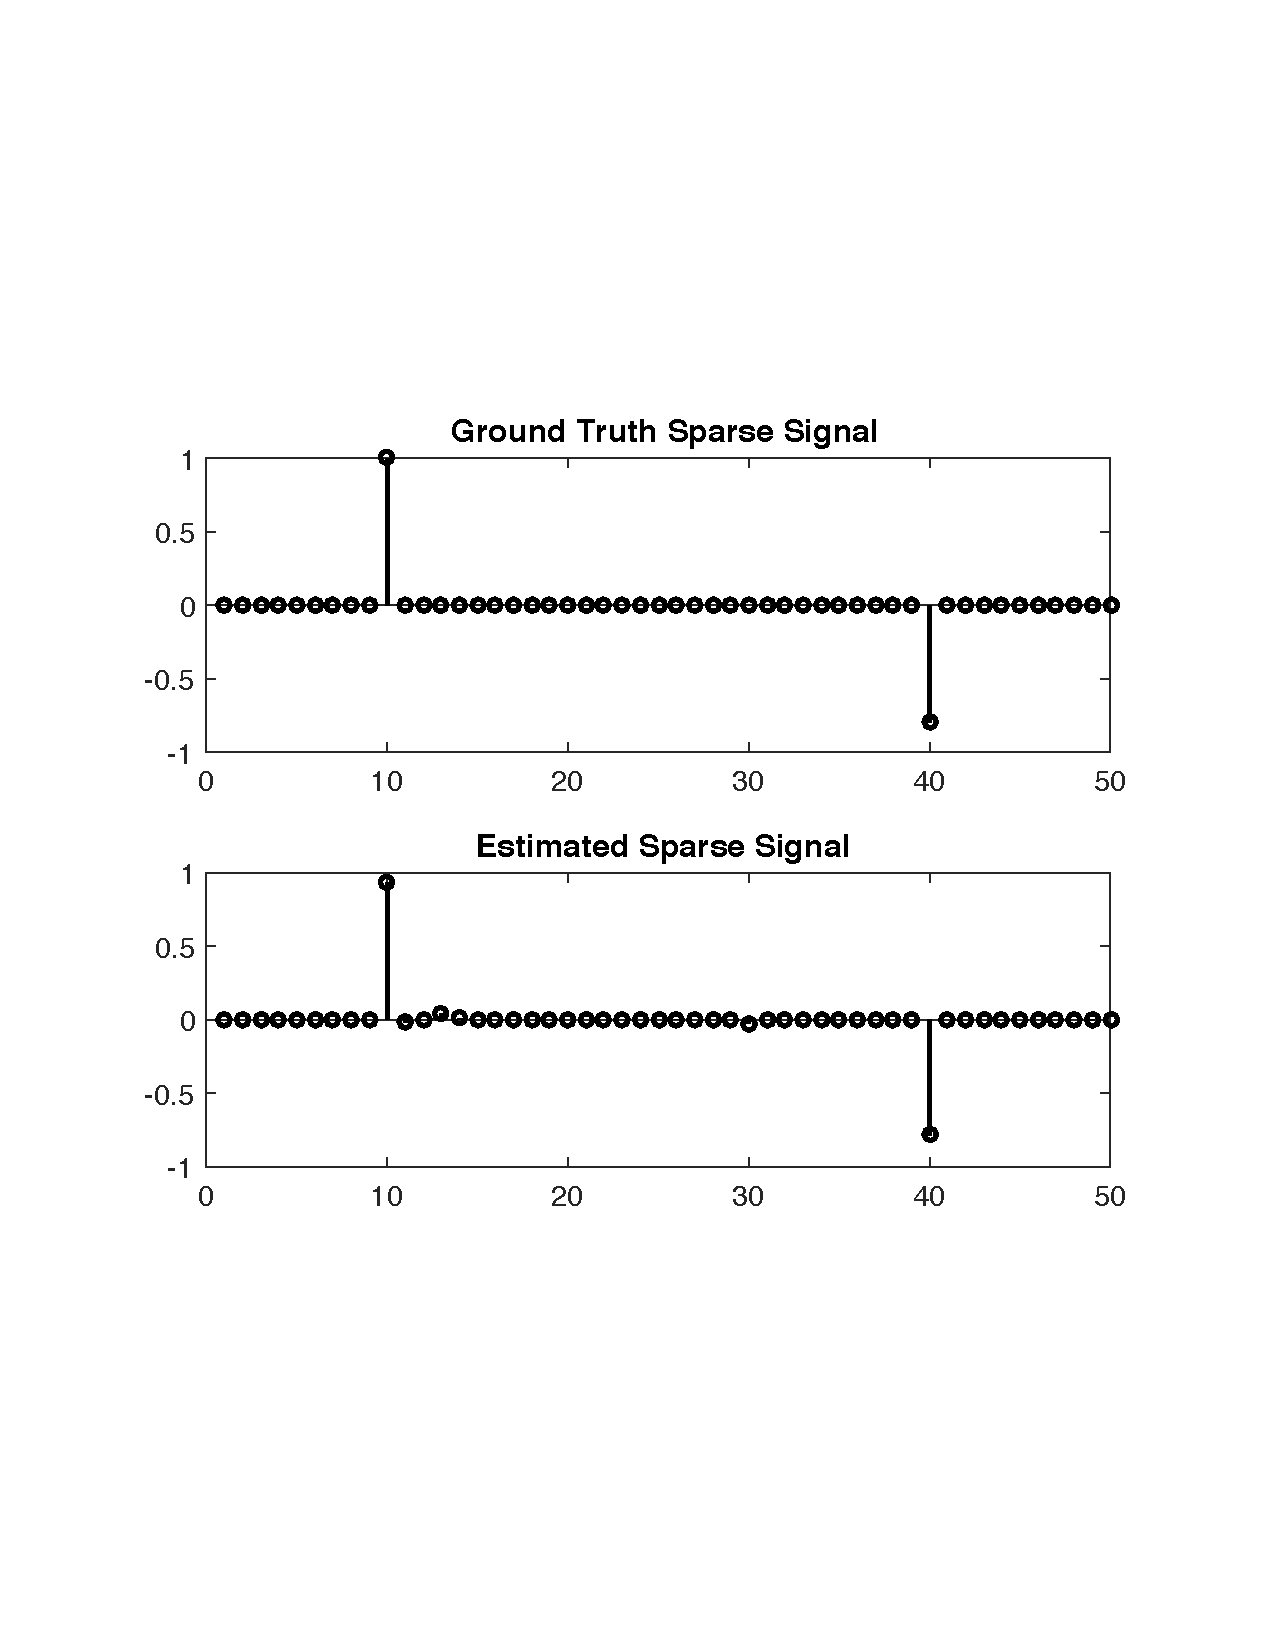
\includegraphics[width=0.95\textwidth]{lassoExample1}
	\captionof{figure}[Example of sparse signal recovery using $\ell_1$ regularized least squares algorithms]{Example of sparse vector recovery using $\ell_1$ regularized least squares algorithms. \gls{snr} = 100. The top plot shows the ground truth signal $\mb{x}$. The bottom plot shows the estimated signal $\mbh{x}$ and $\tau = 0.02$. The number of measurements is $N_m = 10$. The dimensionality of the signal is $N = 50$. }
	\label{fig:lassoExample1}
\end{figure}

\begin{figure}
	\centering
	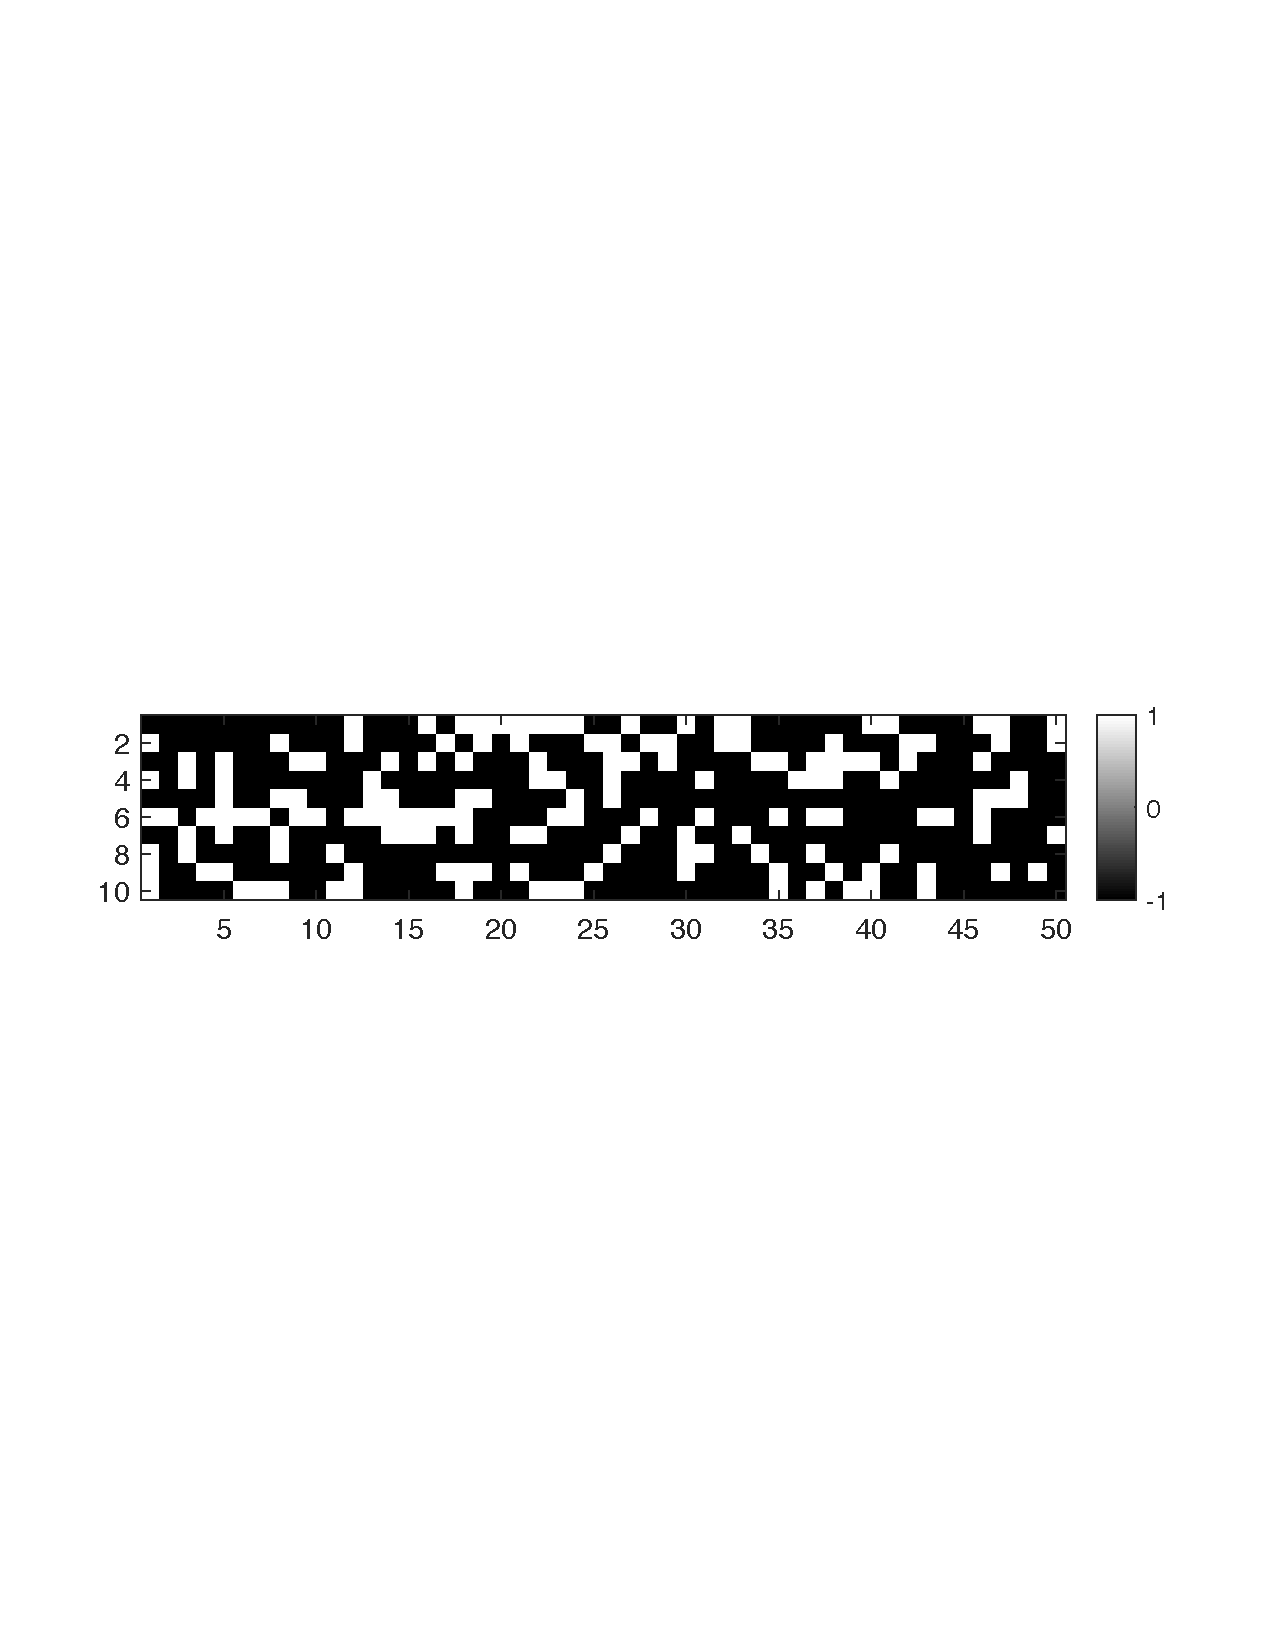
\includegraphics[width=0.95\textwidth]{lassoExample1Matrix}
	\captionof{figure}[The sensing matrix used for \cref{fig:lassoExample1} .]{The sensing matrix $\mb{H}$ used for \cref{fig:lassoExample1}. Since the signal was already sparse, the representation basis can be written as the identity matrix $\mb{\Psi} = \mb{I}$. The number of rows correspond to the number of measurements $N_m$ and the number of columns correspond to the number of elements in the signal vector $\mb{f}$. }
	\label{fig:lassoExample1Matrix}
\end{figure}

%
\begin{figure}
	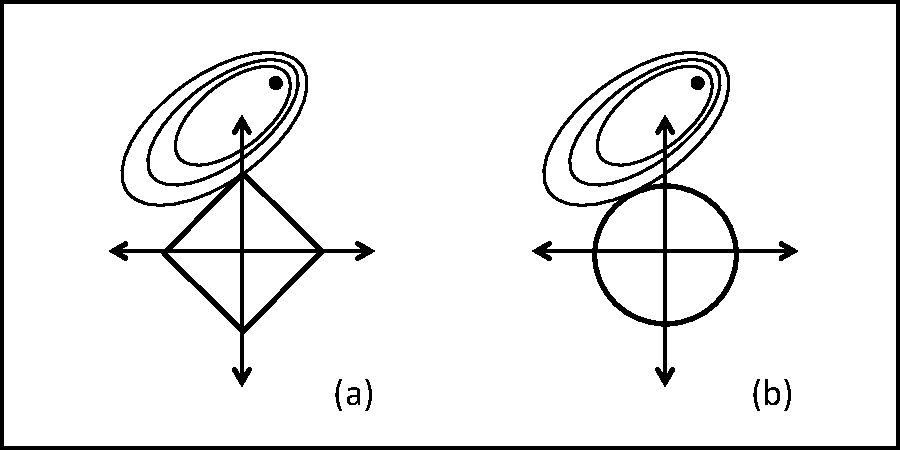
\includegraphics[scale=1]{l1Ball}
	\captionof{figure}[Geometric interpretation of $\ell_1$ regularized least squares.]{(a) $\ell_1$ regularized least squares which is called \gls{lasso} regression. (b) $\ell_2$ regularized least squares which is called ridge regression.}
	\label{fig:l1Ball}
\end{figure}

One can gain some geometric intuition of why the $\ell_1$ regularized least squares produces sparse solutions by looking at \Cref{fig:l1Ball}(a). The dot indicates the unconstrained \gls{ls} solution. The contours represent equal values of the objective function: $\| \mb{Ax} = \mb{g} \|_{2}^{2}$. The solution is when the $\ell_1$ constraint intersects one of the contours. Because of the shape of the $\ell_1$ ball, this tends to occur along one of the coordinate axes. \Cref{fig:l1Ball}(b) represents the situation with $\ell_2$ regularized \gls{ls}, ridge regression, because of the shape of the $\ell_2$ ball the solutions may or may not occur along the coordinate axes.

The \gls{lasso} regression technique in statistics is a way to perform variable selection without overfitting the data \cite{tibshirani1996regression, james2013introduction}. In simple terms, overfitting means that given some seemingly complicated data, overfitting occurs when the model attempts to fit all of the data producing a model with very low error with the given data but will tend to have poor prediction results when new data is obtained. By regularizing the objective function, the model will tend to have better prediction accuracy by producing simpler models even though it may have a larger error trying to fit the current data.

Algorithms for solving the \gls{lasso} improve the accuracy of the estimate by selecting only a subset of the columns of the matrix $A$ which we denote as the $A_s$. An example of the \gls{lar} algorithm which is often used to solve the \gls{lasso} problem is provided in \cite{efron2004least}. By forcing the sum of the absolute value to be less than some fixed value, $\ell_1$ regularized least squares forces certain values of $x_n = 0$, effectively choosing a simpler model out of all the possible solutions provided by \gls{ls}. 

\section{Conclusion}

I used this chapter to cover several important mathematical concepts which are required for the reader to understand the advantages and disadvantages of computational sensing. I first discussed the advantages that Hadamard and S-Matrix multiplexing provided compared to the isomorphic sensor which provided a context for the discussion of the Fellgett advantage. Then I discussed \acrfull{pca}, a useful technique for finding useful discriminating features from seemingly complicated data. I also covered the fundamentals of Bayesian statistics and how it can be used to update estimates of statistical parameters given new data. Then I covered important topics in compressive sensing: sparsity, coherence, and the \acrfull{rip} and discussed the $\ell_1$ regularized \gls{ls} problem which is used to promoted sparsity and has a multitude of algorithms which can be used to solve it. 


%\bibliographystyle{IEEEtranS}  
%\bibliography{ThesisBib}



